\documentclass[12pt, pdf, hyperref={unicode},handout]{beamer}

\mode<presentation>
{
  \usetheme{Madrid}       % or try default, Darmstadt, Warsaw, ... Madrid
  \usecolortheme{default} % or try albatross, beaver, crane, ...default
  \usefonttheme{serif}    % or try default, structurebold, ... serif
  \usefonttheme{professionalfonts}
  \setbeamertemplate{navigation symbols}{}
% \setbeamertemplate{caption}[numbered]
} 

\usepackage[english,russian]{babel}
\usepackage[utf8x]{inputenc}
\usepackage{hyperref}
\graphicspath{{image/}}
\definecolor{links}{HTML}{2A1B81}
\hypersetup{colorlinks,linkcolor=,urlcolor=links}
\usepackage{listings}
\usepackage{concmath}
\usepackage{ragged2e}
\renewcommand{\raggedright}{\leftskip=0pt \rightskip=0pt plus 0cm}
\usepackage[orientation=landscape,size=A4, scale=4]{beamerposter}
\usepackage{enumerate}
\usepackage[T2A]{fontenc}
\usepackage{subfigure}
\usepackage{float}
\usepackage{setspace}
\usepackage{array,longtable}

\lstset{language=R}


% Here's where the presentation starts, with the info for the title slide
\title[Лекция 1]{\Huge{Основные величины и элементы электрических цепей}}
\author[\textcopyright   Артамонов Ю.Н.]{}
\institute[]{}
\date{}

\begin{document}

\begin{frame}
  \titlepage
\end{frame}

% These three lines create an automatically generated table of contents.
\begin{frame}{Содержание}
  \tableofcontents
\end{frame}

\section{Вводные замечания}


\begin{frame}{Историческая справка}
  \begin{block}

    \small{
   Дисциплина <<Электротехника и электроника>> занимает важное место в базовой подготовке специалистов в области информатики и вычислительной техники. Содержание дисциплины составляет изучение процессов, происходящих в различных электротехнических и электронных устройствах, а также принципов построения и использования этих устройств.

Как наука электротехника начала формироваться в середине XIX века. Ее основы заложены в работах Г. Кирхгофа, Г. Ома, М. Фарадея, Дж. Максвелла, Г. Герца. Практическое использование электротехники связано с именами Т. Эдисона, Н. Теслы, П. Н. Яблочкова, М. О. Доливо-Добровольского.

За прошедшие 150 лет электротехника коренным образом изменила жизнь человеческого общества. Электричество стало основой развития промышленности, транспорта, связи, без него невозможна автоматизация производственных процессов. Столь широкому распространению электрической энергии способствовало удобство ее передачи на дальние расстояния и преобразования в другие виды энергии: механическую, тепловую, световую и др.

\textbf{Первые десятилетия ХХ века} ознаменовались развитием радиоэлектроники – области науки и техники, занимающейся исследованием и разработкой устройств, предназначенных для передачи и обработки информации. Началом первого этапа развития радиоэлектроники считается 1904 г., когда английским ученым Д. Флемингом была изготовлена первая электронная лампа – диод. 
}

  \end{block}
  
\end{frame}

\begin{frame}{Историческая справка}
  \begin{block}

    \small{
      Позднее был предложен триод – лампа с управляющим электродом, способная усиливать и генерировать электрические сигналы. Триод стал первым управляемым электронным прибором.

      \textbf{Второй этап} развития радиоэлектроники начался в конце 1940-х гг. с изобретения американскими учеными У. Браттейном, Д. Бардиным и В. Шокли биполярного транзистора. Новый прибор мог усиливать и генерировать электрические сигналы, а также выполнять функции электронного ключа. За это изобретение его создатели были удостоены Нобелевской премии.

Первые транзисторы изготавливали на основе полупроводника германия. Рабочая температура таких приборов не превышала 70 °С. Во многих случаях этого было недостаточно. Во второй половине 1950-х гг. вместо германия стали применять другой полупроводник – кремний. Рабочая температура кремниевых транзисторов составляет 120–150 °С. Кроме того, для кремниевых транзисторов была разработана планарная технология, позволяющая создавать на одной пластине полупроводника тысячи и миллионы транзисторов.
Появление планарной технологии и совершенствование методов выращивания кристаллов кремния привели к созданию в 1960-х годах нового полупроводникового прибора – транзистора со структурой металл – окисел – полупроводник (МОП-транзистора).
}

  \end{block}
  
\end{frame}

\begin{frame}{Историческая справка}
  \begin{block}

    \small{
\textbf{Третий этап} связан с появлением микроэлектроники – направления электроники, охватывающего разработку и производство качественно нового типа приборов – интегральных микросхем. Интегральная микросхема, или просто интегральная схема (ИС), – совокупность большого числа электронных компонентов, изготовленных в едином технологическом цикле на кристалле полупроводникового материала, которая выполняет определенные функции преобразования и обработки сигналов.
Первая цифровая интегральная схема была изобретена в 1959 году и содержала всего 12 транзисторов. Но уже через несколько лет появились большие интегральные схемы (БИС), содержащие тысячи элементов. В настоящее время на кристалле сверхбольшой интегральной схемы (СБИС) расположены десятки миллионов транзисторов, размеры которых составляют менее 0,1 мкм.
В эпоху микроэлектроники кардинально изменилась не только цифровая, но и аналоговая схемотехника. Создание интегральных операционных усилителей связано с именем Р. Видлара, определившего на многие годы структуру аналоговых интегральных схем.
}

  \end{block}
  
\end{frame}

\begin{frame}{Историческая справка}
  \begin{block}

    \small{

Начало 1970-х гг. ознаменовалось созданием микропроцессоров. Они были разработаны фирмой Intel под руководством М. Хоффа. Первый микропроцессор Intel 4004 содержал 2300 транзисторов и работал на частоте 750 кГц. Современные микропроцессоры содержат десятки миллионов транзисторов и работают на частотах, достигающих нескольких ГГц. Они заменяют целые
блоки и устройства радиоэлектронной аппаратуры предшествующих поколений. Благодаря микропроцессорам компьютеры стали массовым, общедоступным продуктом. Микропроцессоры широко используются для автоматизации технологических процессов и в быту.

}

  \end{block}
  
\end{frame}

\begin{frame}{Принятые упрощения}
  \begin{block}

    \small{
      Любой электронный прибор представляет электромагнитное устройство, работу которого можно строго описать методами теории электромагнитного поля. В теории электромагнитного поля оперируют векторными величинами, такими как напряженность электрического поля, магнитная индукция, плотность тока. Методы теории поля дают возможность изучать различные явления в любых электротехнических и электронных устройствах. Однако эти методы сложны и трудоемки даже при решении простых задач.

      Для инженерных расчетов применяют приближенные методы анализа, позволяющие с достаточной степенью точности анализировать поведение электронных и электротехнических устройств. Такие методы дает теория электрических цепей, в которой вместо векторных величин теории поля, зависящих от пространственных координат и времени, используют скалярные величины: ток и напряжение. Для приближенного учета процессов, происходящих в электронных устройствах, в теории цепей введены идеальные элементы. Соединяя между собой эти идеальные элементы, получают схему замещения, или модель, приближенно отображающую процессы в реальном устройстве.

}

  \end{block}
  
\end{frame}

\begin{frame}{Принятые упрощения}
  \begin{block}

    \small{
Методы теории цепей менее универсальны, чем методы теории электромагнитного поля. В частности, их нельзя применять при действии высокочастотных сигналов, когда длина волны электромагнитного колебания сравнима с размерами исследуемого устройства. Тем не менее методы теории цепей широко используют как при ручных расчетах, так и в компьютерных программах моделирования электронных цепей.

Таким образом, теория цепей дает инженерам эффективный инструмент для исследования и проектирования электротехнических и электронных устройств. 
}

  \end{block}
  
\end{frame}

\section{Основные величины электротехники}
\begin{frame}{Электрические и магнитные величины}
  \begin{block}

    \small{
Для количественного и качественного описания электромагнитных явлений применяются электрические и магнитные величины: заряд, ток, напряжение, сопротивление, емкость, индуктивность, магнитный поток, магнитная индукция и др.

Все электрические и магнитные величины однозначно и непротиворечиво могут быть математически выражены только через \textbf{четыре} исходные: \textbf{длину $l$, время $t$, энергию $w$ и электрический заряд $q$, а также через дополнительную величину - угол $\varphi$}. Однако в электротехнике используют производные от этих физических величин: \textbf{электрический ток, напряжение, мощность}.
При описании электромагнитных процессов электрическими цепями по т.радиции используется термин электрическая энергия. В электротехнике, электроснабжении и других отраслях техники для сокращения используется термин электроэнергия.

Энергия обозначается буквой $w$ ($W$) и измеряется в джоулях (Дж). (все электрические величины, являющиеся функциями времени называются мгновенными значениями, обозначаются строчными буквами: $w(t), q(t), u(t), p(t), e(t), i(t)$. Электрические величины, имеющие постоянные значения, обозначаются прописными буквами: $W, Q, U, P, E, I$ и т.д.) При любых физических процессах соблюдается закон сохранения и превращения энергии. На основе этого закона анализируются методы получения электрической энергии из других ее видов в соответствующих устройствах, называемых источниками электрической энергии (электромашинные генераторы, магнитогидродинамические генераторы, аккумуляторы и т.п.).

}

  \end{block}
  
\end{frame}

\begin{frame}{Электрический ток}
  \begin{block}

    \small{
\textit{Электрический ток} - это скорость изменения заряда во времени. Электрический ток обозначается буквой $i (I)$ и измеряется в амперах (А): $$i(t)=\frac{d q(t)}{d t}$$
Токи, зависящие от времени, называются \textit{переменными токами}, например: $$i(t)=I_m\sin(wt+\varphi)$$
Если мгновенное значение тока постоянно в любой момент времени t, то такие токи называются \textit{постоянными} и обозначаются прописными буквами $I$. Для измерения электрического тока применяются специальные приборы \textit{амперметры}, включаемые \textbf{последовательно с измеряемым током}. Электрический ток на схемах обозначается стрелкой, поставленной на проводе.
\begin{figure}[htb] 
    \centering
    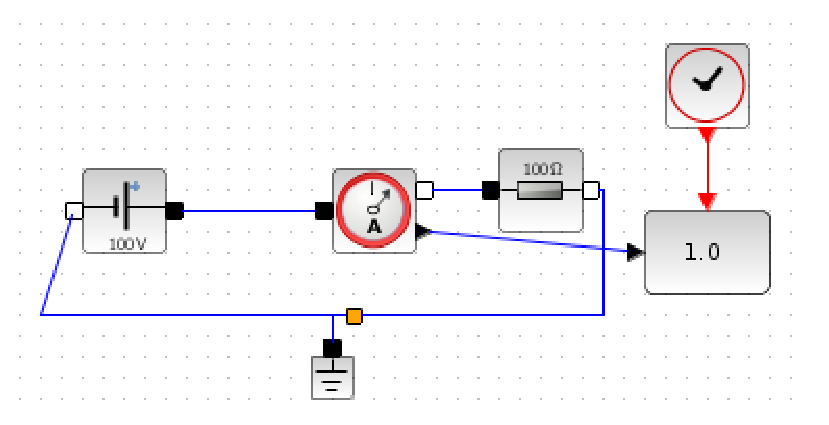
\includegraphics [scale=0.9]{ris1.eps}
  \end{figure}

}

  \end{block}
  
\end{frame}

\begin{frame}{Электромагнитная мощность}
  \begin{block}

    \small{
\textit{Электромагнитная мощность} - это скорость изменения электромагнитной энергии во времени. Электромагнитная мощность  обозначается буквой $p (P)$ и измеряется в ваттах (Вт): $$p(t)=\frac{d w(t)}{d t}$$
Мощность измеряется ваттметрами. Мощность приемников всегда положительна.

Для расчета или измерения мощности знание или измерение только тока недостаточно. Необходима еще одна электрическая величина, учитывающая разное <<удельное электрическое усилие>>, <<электрическое напряжение>>, <<прикладываемое>> к приемникам с различной мощностью при одинаковом токе.


}

  \end{block}
  
\end{frame}

\begin{frame}{Электрическое напряжение}
  \begin{block}

    \small{
Для характеристики качественной связи между мощностью и током, а также для определения количественного соотношения между мощностью и током используется физическая величина
\textit{электрическое напряжение}.

\textit{Электрическое напряжение}  равно отношению электрической мощности (скорости поглощения электромагнитной энергии, ее преобразования в другие виды энергии) к электрическому току: $$u(t)=\frac{p(t)}{i(t)}$$
Напряжение обозначается буквой $u (U)$ и измеряется в вольтах [В]= [Вт/А]. На схемах напряжение обозначается стрелкой расположенной рядом с приемником энергии и направленной согласно с направлением тока, т. е. от большего потенциала к меньшему. Для анализа и измерения электрического напряжения применяются \textbf{осциллографы и вольтметры}. Они включаются в схему одинаково: к выводам приемника или источника электрической энергии (\textbf{параллельно}).
\begin{figure}[htb] 
    \centering
    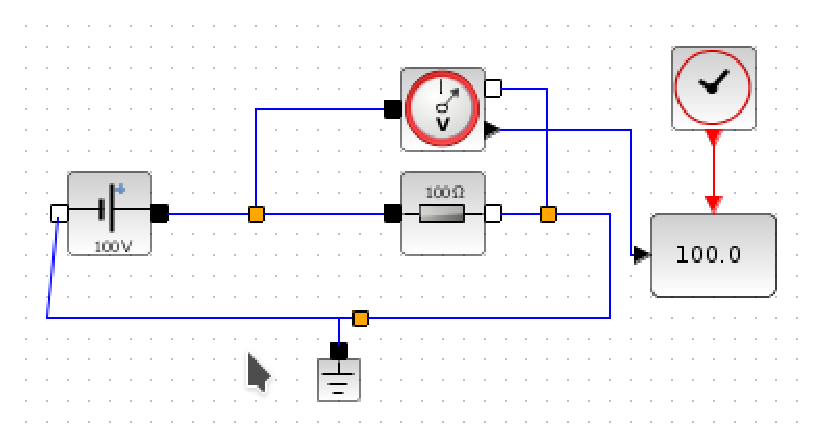
\includegraphics [scale=0.7]{ris2.eps}
  \end{figure}

}

  \end{block}
  
\end{frame}

\begin{frame}{Электрическое сопротивление и проводимость}
  \begin{block}

    \small{
      \textit{Свойство вещества проводить под действием не изменяющегося во времени электрического поля не изменяющийся во времени электрический ток называется \textbf{электропроводностью.}}
      
      Вещества, обладающие электропроводностью, называются \textbf{проводниками}. К ним относятся, например, металлы: медь, серебро, алюминий, железо, и их сплавы.

      Вещества, не обладающие электропроводностью, называются \textbf{диэлектриками}. Ими является большое количество различных неорганических и органических материалом.

      В современной технике большое применение нашли вещества, которые нельзя отнести ни к проводникам, ни к диэлектрикам - это большая группа \textbf{полупроводниковых материалов} с сильной зависимостью электропроводности от внешних факторов: температуры, электрического поля, света и т.д. Также уделяется внимание газам, коллоидным растворам, электропроводность которых также зависит от внешних условий (температуры, давления и т.д.). Интенсивно изучается такое явление, как \textbf{сверхпроводимость}, т.е. полное отсутствие сопротивления проводника. Она обнаруживается у ряда веществ при температуре, близкой к абсолютному нулю.

      В целом для качественной и количественной характеристики электропроводности используется физическая величина - \textbf{электрическое сопротивление}.

}

  \end{block}
  
\end{frame}

\begin{frame}{Электрическое сопротивление и проводимость}
  \begin{block}

    \small{
      Электрическое сопротивление проводника определяется как отношение мощности потерь электромагнитной энергии в нем к квадрату электрического тока: $$R=\frac{p(t)}{i^2(t)}$$
      При постоянной токе $$R=\frac{P}{I^2}$$
      На практике более удобно выражать сопротивление через напряжение:
      $$R=\frac{P}{I^2}=\frac{UI}{I^2}=\frac{U}{I}$$
      У проводников потери электромагнитной энергии при постоянном токе относительно невелики. Немецкий физик Ом, проводя эксперименты и измеряя токи проводников при различных напряжениях, пришел к выводу, что их сопротивление не зависит от приложенного напряжения и является постоянной величиной. Этот факт известен как \textbf{закон Ома}: $U=RI, R=const$
      
      Сопротивление обозначается буквой $R$ и измеряется в омах [Ом]. Электрическое сопротивление характеризует процесс безвозвратного преобразования электромагнитной энергии в другие виды (в основном в теплоту).

}

  \end{block}
  
\end{frame}

\begin{frame}{Электрическое сопротивление и проводимость}
  \begin{block}

    \small{
      \textit{Величина, обратная сопротивлению, называется \textbf{электрической проводимостью}.} Проводимость обозначается буквой $G$ и измеряется в \textbf{сименсах} [См]=[1/Ом]=[A/B]:
      $$G=\frac{1}{R}=\frac{I}{U}$$
      Проводимость характеризует электропроводность проводников: чем больше проводимость, тем лучше электропроводность.

      Как было установлено позже, закон Ома является относительным и может выполняться только в определенных условиях, однако само соотношение $U=RI$ является универсальным, справедливым для любых электромагнитных процесов только с потерями энергии, без ее накопления.

      Как показали многочисленные эксперименты, сопротивление проводников изменяется в зависимости от температуры. Для многих металлов эта зависимость носит линейный характер: $R(t)=R_0(1+\alpha (t-t_0)),$ где $R_0$ - сопротивление проводника при температуре $t_0$, $\alpha$ - коэффициент, называемый температурным коэффициентом сопротивления (обычно у металлов он достаточно мал). Сопротивление проводника также зависит от его геометрических размеров: $R=\frac{\rho\cdot l}{S}$, где $l$ - длина проводника, $S$ - площадь поперечного сечения, $\rho$ - удельное сопротивление, характеризующее электропроводность данного металла.
    }

  \end{block}
  
\end{frame}

\section{Основные элементы электротехники}

\subsection{Источники напряжения, тока}
\begin{frame}{Электродвижущая сила источника энергии}
  \begin{block}

    \small{
      Для производства электроэнергии тепловые, атомные, гидроэлектростанции, а также гальванические элементы и аккумуляторы. Их способность вырабатывать электрическую энергию количественно характеризуется \textbf{электродвижущей силой (ЭДС)}, которая равна отношению электрической мощности источника к его току:
      $$e(t)=\frac{p(t)}{i(t)}$$
      Электрическое напряжение и ЭДС характеризуют противоположные электрические процессы: положительному напряжению соответствует процесс преобразования электрической энергии в другие виды энергии, а положительной ЭДС соответствует процесс производства электрической энергии из других видов.
      В целом производство и потребление электроэнергии  - это единый процесс: в любой момент источник вырабатывает ровно столько энергии, сколько ее потребляет приемник. При этом производство электрической энергии в источниках сопровождается потерями части произведенный энергии внутри самого источника, которые определяются его \textbf{внутренним сопротивлением}.
    В зависимости от соотношения между внутренним сопротивлением и сопротивлением нагрузки источники электрической энергии идеализированно представляются либо \textbf{источниками напряжения}, либо \textbf{источниками тока}.  
}

  \end{block}
  
\end{frame}


\begin{frame}{ Источник напряжения}
  \begin{block}

    \small{
      \textit{У источника напряжения на выходах поддерживается постоянное напряжение при изменении нагрузки в достаточно широких пределах: $U_{\text{вых}}=E=const.$}

      Мощность источника напряжения прямо пропорциональна току нагрузки: $P=E\cdot I, E=const.$ На рисунке показана \textbf{вольт-амперная характеристика (ВАХ)} источника напряжения: зависимость напряжения на выходах  от тока.
      \begin{figure}[htb] 
    \centering
    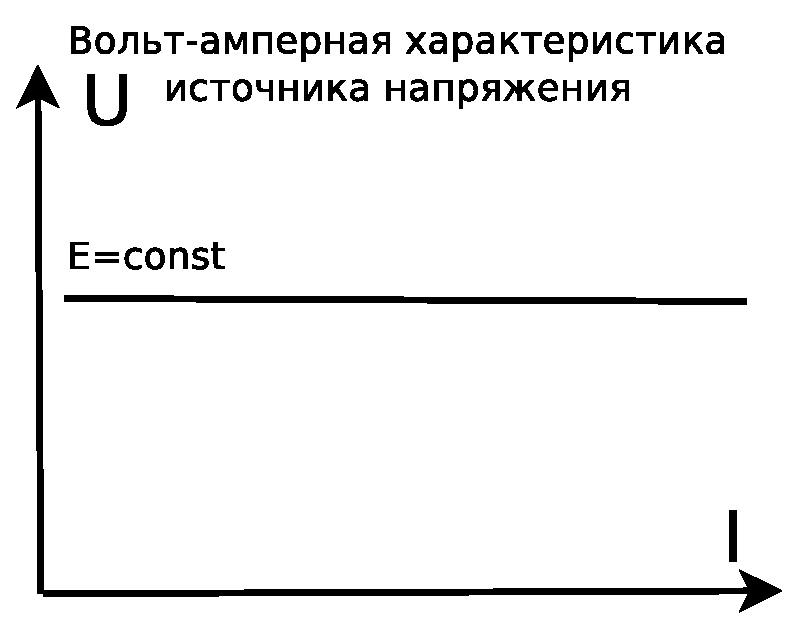
\includegraphics [scale=0.7]{ris3.eps}
  \end{figure}
  $U=E=R_{\text{внут}}I\Rightarrow R_{\text{внут}}=\frac{\Delta U}{\Delta I}=\frac{0}{\Delta I}=0$. Таким образом, внутреннее сопротивление источника напряжения принято считать равным нулю.

  
}

  \end{block}
  
\end{frame}

\begin{frame}{ Источник напряжения}
  \begin{block}

    \small{
      Например, выходное напряжение свинцовых аккумуляторов при изменении тока практически остается постоянным. Это означает, что такой аккумулятор имеет очень малое внутреннее сопротивление (поэтому если его закоротить, потечет очень большой ток). Источники напряжения на схемах обозначаются кружком со стрелкой (при стрелке показана положительная полярность).      
      \begin{figure}[htb] 
    \centering
    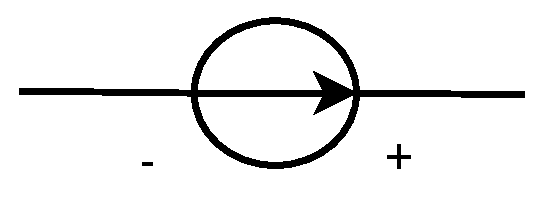
\includegraphics [scale=0.7]{ris4.eps}
  \end{figure}

  Мы также будем использовать обозначение в системе scilab (предполагается, что на выходе 9 вольт).
  \begin{figure}[htb] 
    \centering
    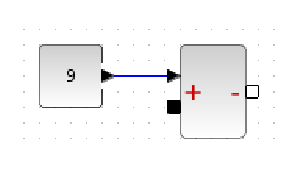
\includegraphics [scale=1]{ris5.eps}
  \end{figure}

  
}

  \end{block}
  
\end{frame}

\begin{frame}{ Источник тока}
  \begin{block}

    \small{
      Другой моделью источников электрической энергии является \textbf{источник тока}, у которого при изменении сопротивления нагрузки его ток постоянен:$\frac{P}{U}=I=const$. На рисунке показана ВАХ источника тока. $R_{\text{внут}}=\frac{\Delta U}{\Delta I}=\frac{\Delta U}{0}=\infty$
  \begin{figure}[htb] 
    \centering
    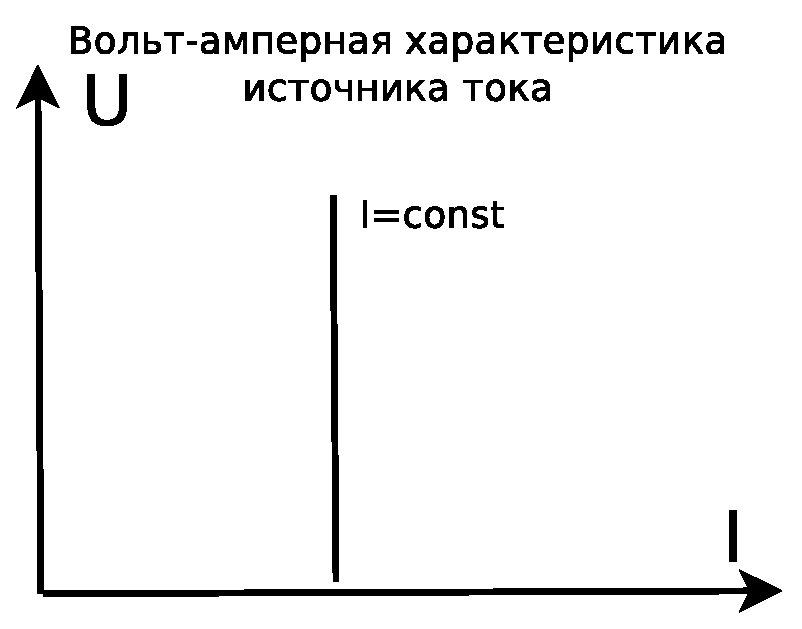
\includegraphics [scale=0.6]{ris6.eps}
  \end{figure}
  Таким образом, внутреннее сопротивление источника тока можно считать бесконечно большим (такой источник должен находиться под нагрузкой, или быть закорочен(в этом случае $U_{\text{вых}}=0$ и мощность равна нулю)).
  Условное обозначение источников тока показано на рисунке:
\begin{figure}[htb] 
    \centering
    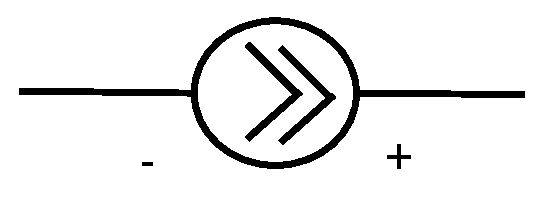
\includegraphics [scale=0.6]{ris7.eps}
    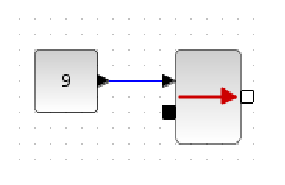
\includegraphics [scale=0.8]{ris8.eps}
  \end{figure}
  На последнем рисунке предполагается, что источник тока выдает 9 А.
}

  \end{block}
  
\end{frame}

\begin{frame}{Реальные источники электрической энергии}
  \begin{block}

    \small{
      Источники напряжения и тока - это идеализированные элементы. На практике источники электрической энергии обладают внутренним сопротивлением отличным от нуля или бесконечности. За счет этого производство электрической энергии сопровождается потерей ее части внутри самого источника. Для учета этого обстоятельства используют две схемы замещения для реального источника электрической энергии: схема замещения на основе источника напряжения, схема замещения на основе источника тока.
      \textit{Внутренние потери электроэнергии источника напряжения учитываются внутренним сопротивлением $R_{\text{вн}}$, соединенным последовательно с источником напряжения:
\begin{figure}[htb] 
    \centering
    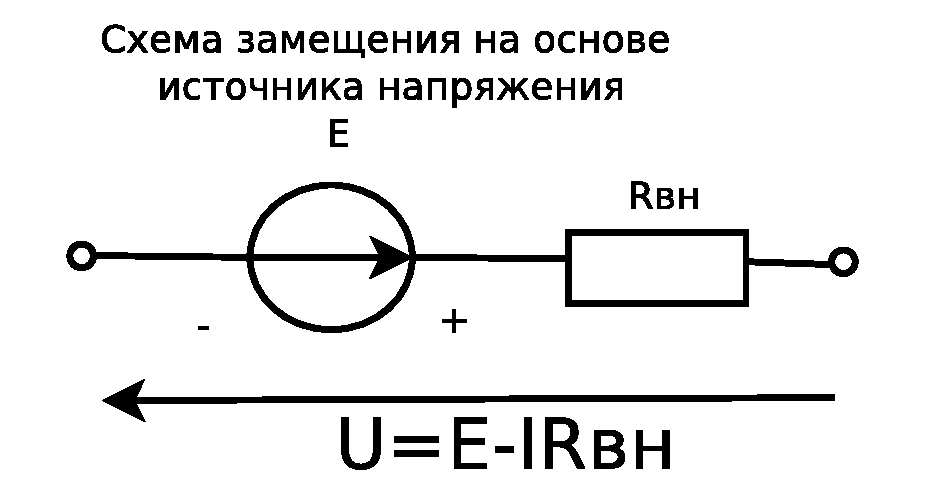
\includegraphics [scale=0.6]{ris9.eps}
    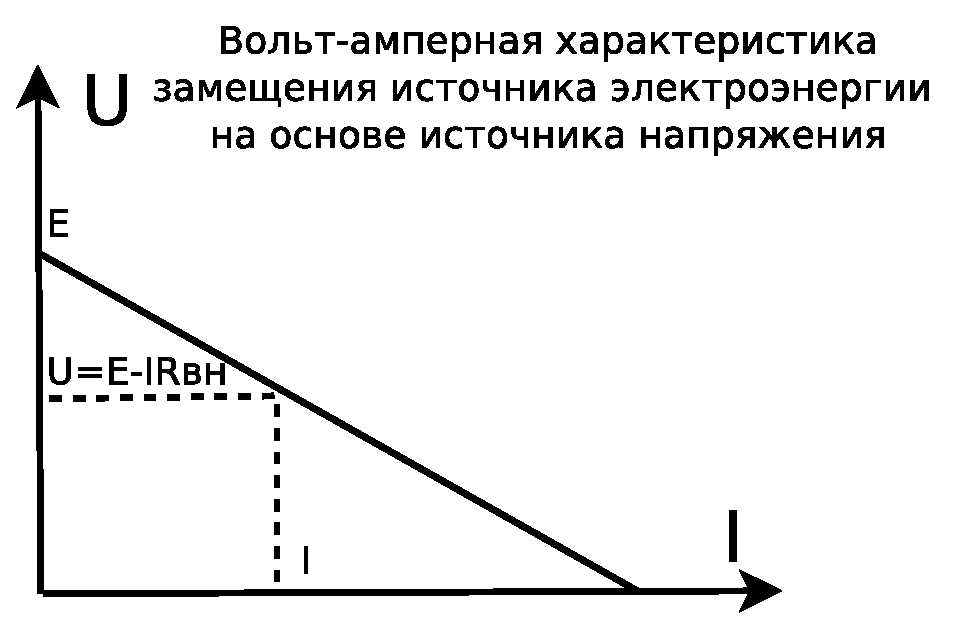
\includegraphics [scale=0.6]{ris10.eps}
  \end{figure}
 При наличии тока нагрузки $I$ выходное напряжение источника меньше, чем ЭДС $E$, на падение напряжения на внутреннем сопротивлении:  $$U=E-R_{\text{вн}}\cdot I$$ 
      }
}

  \end{block}
  
\end{frame}

\begin{frame}{Реальные источники электрической энергии}
  \begin{block}

    \small{
      \textit{Внутренние потери электроэнергии источника тока учитываются внутренней проводимостью $G_{\text{вн}}$, соединенной параллельно с источником тока:
\begin{figure}[htb] 
    \centering
    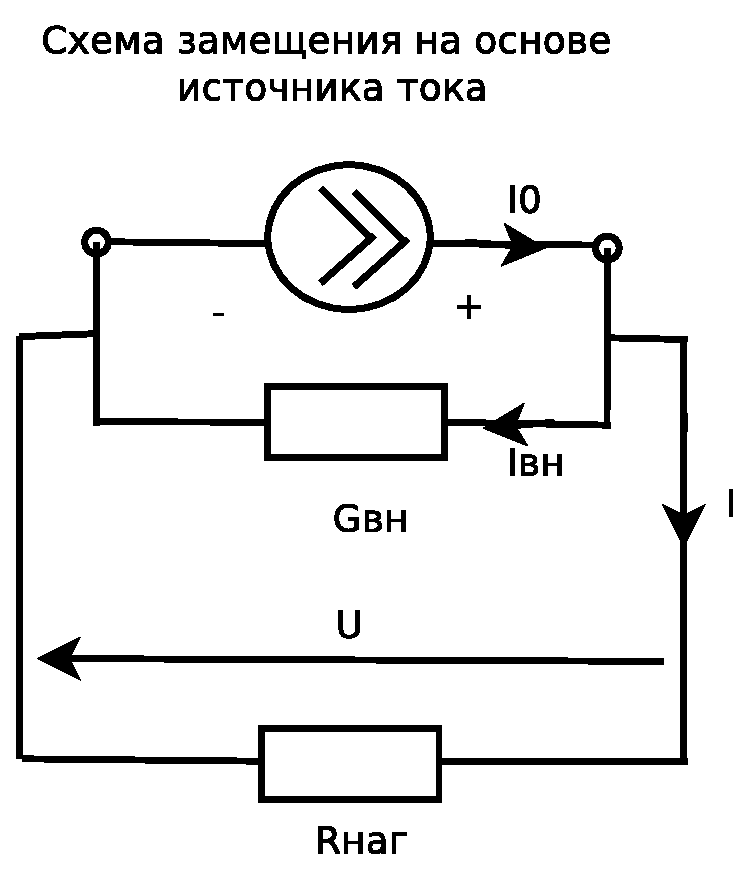
\includegraphics [scale=0.6]{ris11.eps}
  \end{figure}
  При наличии тока нагрузки $I$ выходное напряжение определяется:
  $$I_o=I+I_{\text{вн}}=I+UG_{\text{вн}}$$
  $$U=\frac{I_0}{G_{\text{вн}}}-\frac{I}{G_{\text{вн}}}$$
      }
}

  \end{block}
  
\end{frame}

\subsection{Резистивный элемент}
\begin{frame}{Резистивный элемент}
  \begin{block}

    \small{
\textbf{Резистивным элементом $R$} называют идеализированный двухполюсный элемент,
для которого связь между напряжением, приложенным к этому резистивному элементу $U$, и током через него $I$ удовлетворяет закону Ома: $U=R\cdot I$ .
Резистивный элемент моделирует процесс необратимого преобразования электромагнитной
энергии в тепло и другие виды энергии, при этом запасание энергии в электромагнитном поле отсутствует.
На схемах резистивный элемент обозначается следующим образом:
\begin{figure}[htb] 
    \centering
    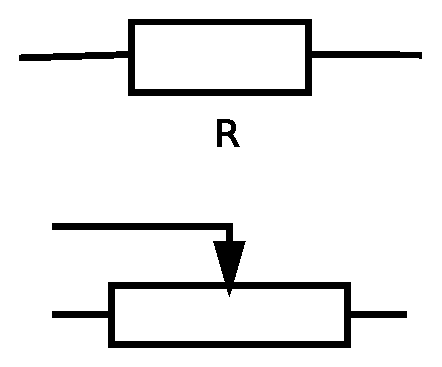
\includegraphics [scale=0.6]{ris12.eps}
  \end{figure}
  Для практической реализации линейного сопротивления промышленность изготавливает специальные радиодетали: \textbf{резисторы}. Линейные нерегулируемые резисторы характеризуются двумя параметрами: номинальным значением сопротивления (с определенным допуском в процентах) и максимальным значением мощности рассеяния (мощности, до которой резистор не меняет своих электрических свойств и считается идеальным резистивным элементом).
}

  \end{block}
  
\end{frame}

\begin{frame}{Резистивный элемент}
  \begin{block}

    \small{
Внешний вид резисторов показан на фото
  \begin{figure}[htb] 
    \centering
    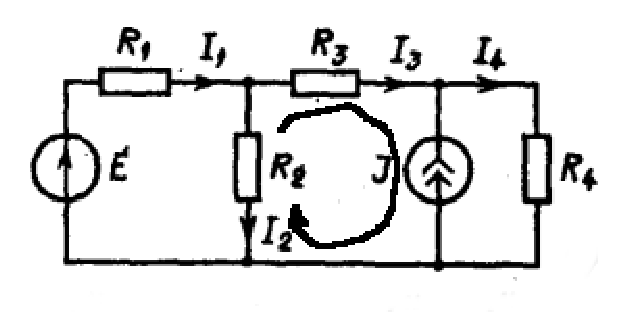
\includegraphics [scale=0.1]{ris13.eps}
  \end{figure}
}

  \end{block}
  
\end{frame}

\section{Схемы электрических цепей}
\begin{frame}{Схемы электрических цепей}
  \begin{block}

    \small{
      Электрическая цепь является моделью электромагнитных процессов.
      \textit{Графическое изображение электрической цепи, содержащее условные обозначения ее элементов и показывающее соединение этих элементов, называется схемой электрической цепи.}

      Схема электрической цепи позволяет математически описать процессы на основе математического аппарата: законов, правил и математических соотношений, а также реализовать ее физическую модель из ограниченного числа электротехнических приборов и деталей. 
}

  \end{block}
  
\end{frame}



\section{Используемая среда Scilab}
\begin{frame}{}
  \begin{block}

    \small{
      Для реализации различных схем электрических цепей в курсе мы будем использовать систему Scilab (инструмент визуального моделирования xcos). Ниже представлены основные ссылки:
      
      \href{https://ru.wikipedia.org/wiki/Scilab}{Информация из википедии}

      \href{https://www.scilab.org/}{Официальный сайт}

      \href{https://online-electric.ru/virtlab.php}{Альтернативные варианты}
      
}

  \end{block}
  
\end{frame}


\end{document}
